\documentclass[11pt]{article}

\usepackage[margin=1in]{geometry}
\usepackage{amsmath, amssymb, bm}
\usepackage{graphicx}
\usepackage{caption, subcaption}
\usepackage{booktabs}
\usepackage{enumitem}
\usepackage{listings}
\usepackage{xcolor}
\usepackage[hidelinks]{hyperref}
\usepackage{fancyhdr}

\graphicspath{{figures/}}

\pagestyle{fancy}
\fancyhf{}
\lhead{MTE 544 -- Assignment 2}
\rhead{Arjun Mandair}
\cfoot{\thepage}

\lstset{
  language=Python,
  basicstyle=\ttfamily\small,
  keywordstyle=\color{blue},
  commentstyle=\color{gray},
  stringstyle=\color{teal},
  numbers=left,
  numberstyle=\tiny,
  breaklines=true,
  frame=single
}

% Handy shortcuts
\newcommand{\vect}[1]{\mathbf{#1}}
\newcommand{\mat}[1]{\mathbf{#1}}

\title{MTE 544 -- Autonomous Mobile Robots\\Assignment 2}
\author{Arjun Mandair \\ Student ID: \texttt{21028006}}
\date{Due November 13, 2026}

\begin{document}
\maketitle
\thispagestyle{fancy}

% =====================================================================
\clearpage
\section{RANSAC with Ellipse I (18 pts)}

\subsection*{1(a) Minimum number of points and construction method [10 pts]}

The ellipse is written as
\begin{equation*}
    Ax^2 + 2Bxy + Cy^2 - 2Dx - 2Ey + 1 = 0.
\end{equation*}
A conic has 6 coefficients but only 5 degrees of freedom, because multiplying the whole equation by any nonzero number gives the same curve. Fixing the constant term at 1 removes that scaling, which leaves 5 unknowns, $\bm{\theta} = [A, B, C, D, E]^\top$. The matrix form gives the same count: $\mat{Q}$ is symmetric, so it has 3 independent entries, and $\vect{b}$ has 2, for 5 in total.

Substituting a data point $\vect{p}_i = (x_i, y_i)$ turns every $x$ and $y$ into a known number. Moving the 1 to the right-hand side then gives one equation that is linear in $\bm{\theta}$:
\begin{equation*}
    x_i^2\,A + 2x_iy_i\,B + y_i^2\,C - 2x_i\,D - 2y_i\,E = -1.
\end{equation*}
Five points give five such equations. Stacking them gives
\begin{equation*}
    \mat{M}\bm{\theta} = -\vect{1}, \qquad -\vect{1} = [-1, -1, -1, -1, -1]^\top \in \mathbb{R}^5,
\end{equation*}
where row $i$ of $\mat{M}$ is $[x_i^2,\ 2x_iy_i,\ y_i^2,\ -2x_i,\ -2y_i]$.

\begin{itemize}
    \item \textbf{Fewer than 5 points:} the system is underdetermined, so it has infinitely many solutions (conics), or none.
    \item \textbf{Exactly 5 points:} this is the minimum. There is a unique solution $\bm{\theta} = \mat{M}^{-1}(-\vect{1})$ whenever $\mat{M}$ is invertible (rank 5).
\end{itemize}

Solving in polynomial form is useful because the unknowns appear linearly, so fitting reduces to solving a linear system. The $(\mat{Q}, \vect{b})$ form is easier to interpret ($\vect{b}$ is the centre, $\mat{Q}$ sets the size and orientation), but it isn't linear in its unknowns.

\subsubsection*{Method to construct the ellipse}
\begin{enumerate}
    \item Build $\mat{M}$ from the 5 points and solve $\mat{M}\bm{\theta} = -\vect{1}$ for $A, B, C, D, E$.
    \item Let $\mat{N} = \begin{bmatrix} A & B \\ B & C \end{bmatrix}$ and $\vect{d} = [D, E]^\top$. The handout gives $\mat{Q} = \alpha\mat{N}$ and $\mat{Q}\vect{b} = \alpha\vect{d}$. Substituting the first relation into the second gives $\alpha\mat{N}\vect{b} = \alpha\vect{d}$, so $\vect{b} = \mat{N}^{-1}\vect{d}$.
    \item Compute $\alpha = 1 / (\vect{d}^\top\mat{N}^{-1}\vect{d} - 1)$, then $\mat{Q} = \alpha\mat{N}$.
    \item Check that $\mat{Q}$ is positive definite (both eigenvalues $> 0$). If it is, the result is an ellipse. If not, it is a hyperbola or a degenerate conic, and the 5 points are rejected.
\end{enumerate}

\subsubsection*{Assumptions and failure cases}
\begin{itemize}
    \item \textbf{The ellipse does not pass through the origin.} Fixing the constant at 1 requires the true constant to be nonzero. A conic through $(0, 0)$ has a constant term of 0, so it cannot be scaled to 1. In that case $\mat{M}$ is singular (rank 4) and the method fails.
    \item \textbf{No 4 of the 5 points are collinear.} Four points on one line make $\mat{M}$ singular, because infinitely many line-pair conics fit them.
    \item 3 collinear points (with no 4 collinear) still leave $\mat{M}$ invertible, but the unique solution is a degenerate pair of lines. A degenerate conic satisfies $\det(\mat{N})\,(1 - \vect{d}^\top\mat{N}^{-1}\vect{d}) = 0$, so for intersecting lines ($\mat{N}$ invertible) $\vect{d}^\top\mat{N}^{-1}\vect{d} = 1$ and $\alpha$ is undefined: the sample is rejected at step 3. For parallel lines, $\mat{N}$ is singular (next case).
    \item $\mat{N}$ is singular (the parabola case, $AC - B^2 = 0$): $\mat{N}^{-1}$ does not exist, so reject the sample.
    \item $\vect{d}^\top\mat{N}^{-1}\vect{d} = 1$: $\alpha$ is undefined (division by zero), so reject the sample.
\end{itemize}
The checks in the last two bullets run before step 4, so they need their own guards. In code, \texttt{fit\_ellipse\_subset} raises \texttt{LinAlgError} for these cases, and \texttt{ransac\_ellipse} catches it and skips that sample.

\subsection*{1(b) Ellipse fit to the given dataset [8 pts]}

The method from 1(a) was applied in Python (\texttt{MTE\_544\_AS2\_Q1\_ArjunMandair.py}) to the points
\begin{equation*}
    (2.92, -6.01), \quad (3.40, -7.20), \quad (4.99, -7.84), \quad (5.48, -7.04), \quad (4.20, -5.91).
\end{equation*}
The resulting $\mat{M}$ has rank 5, so the solution is unique. Values are rounded to 8 decimal places for display. The handout does not specify units for the data, so all coordinates are treated as unitless.

\begin{center}
\begin{tabular}{ll}
    \toprule
    Parameter & Value \\
    \midrule
    $A$ & $0.01806282$ \\
    $B$ & $0.01206936$ \\
    $C$ & $0.03015325$ \\
    $D$ & $-0.00624961$ \\
    $E$ & $-0.15441197$ \\
    $\vect{d}^\top\mat{N}^{-1}\vect{d}$ & $1.02399341$ \\
    $\alpha$ & $41.67811288$ \\
    \bottomrule
\end{tabular}
\end{center}

\begin{equation*}
    \mat{Q} = \begin{bmatrix} 0.75282437 & 0.50302811 \\ 0.50302811 & 1.25673065 \end{bmatrix},
    \qquad
    \vect{b} = \begin{bmatrix} 4.19868909 \\ -6.80150371 \end{bmatrix}.
\end{equation*}

The eigenvalues of $\mat{Q}$ are $0.44217849$ and $1.56737653$. Both are positive, so $\mat{Q}$ is positive definite and the conic is an ellipse. As a check, all five points give $(\vect{p}_i - \vect{b})^\top\mat{Q}(\vect{p}_i - \vect{b}) = 1.000000$, and $\mat{Q}\vect{b} = \alpha\vect{d} = [-0.26047206,\ -6.43559953]^\top$.

\begin{figure}[h!]
    \centering
    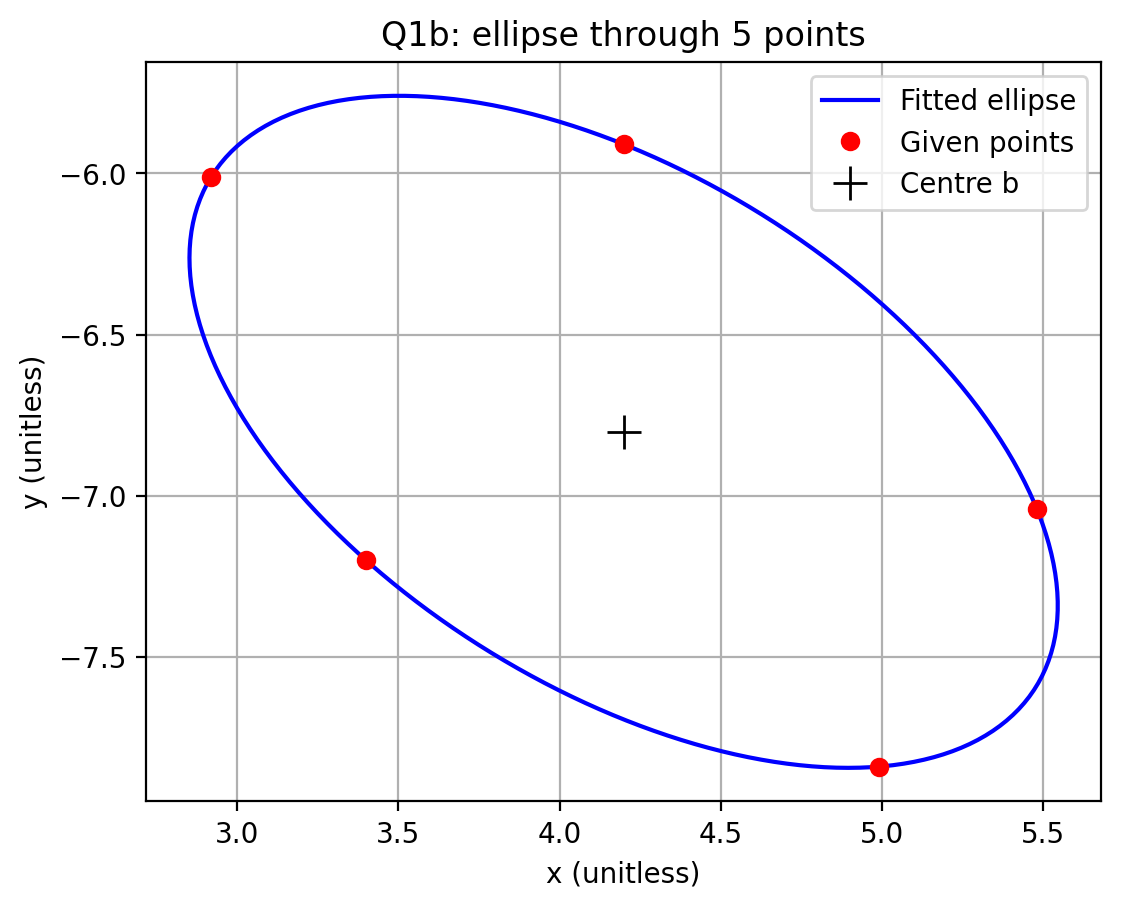
\includegraphics[width=0.7\linewidth]{q1b_ellipse.png}
    \caption{Ellipse fitted through the five given points, with centre $\vect{b}$. The handout does not specify units for the data, so the axes are unitless.}
    \label{fig:q1b}
\end{figure}


% =====================================================================
\clearpage
\section{RANSAC with Ellipse II (30 pts)}

\subsection*{2(a) \texttt{fit\_ellipse\_subset} [8 pts]}

The Q2 script implements \texttt{fit\_ellipse\_subset} using the 5-point method from 1(a). Applied to the five points from 1(b), it gives
\begin{equation*}
    \mat{Q} = \begin{bmatrix} 0.75282437 & 0.50302811 \\ 0.50302811 & 1.25673065 \end{bmatrix},
    \qquad
    \vect{b} = \begin{bmatrix} 4.19868909 \\ -6.80150371 \end{bmatrix},
\end{equation*}
which matches 1(b), and all five points give $(\vect{p}_i - \vect{b})^\top\mat{Q}(\vect{p}_i - \vect{b}) = 1$.

\subsection*{2(b) \texttt{ransac\_ellipse} [12 pts] \quad (max 150 words)}

For \texttt{num\_iterations} rounds:
\begin{enumerate}
    \item Sample 5 distinct random points, the minimum that defines an ellipse (Q1a).
    \item Fit $\mat{Q}$ and $\vect{b}$ with \texttt{fit\_ellipse\_subset}. If $\mat{M}$ or $\mat{N}$ is singular or $\alpha$ is undefined, the fit raises an error and the sample is skipped.
    \item Reject the fit if $\mat{Q}$ is not positive definite, since it is then a hyperbola or degenerate conic, not an ellipse.
    \item Reject the fit if its centre $\vect{b}$ lies outside the data's bounding box or its largest semi-axis ($1/\sqrt{\lambda}$) exceeds the data's span. The handout's inlier test is relative to ellipse size, so very large ellipses would otherwise count most points as inliers and win.
    \item Mark point $\vect{p}_i$ as an inlier if $\left|\sqrt{(\vect{p}_i - \vect{b})^\top\mat{Q}(\vect{p}_i - \vect{b})} - 1\right| \leq \varepsilon$.
    \item If this model has more inliers than the best so far, store its $\mat{Q}$, $\vect{b}$ and inliers.
\end{enumerate}
Return the model with the most inliers (maximum consensus).

\subsubsection*{Result}
One run with the template's default settings ($N = 500$ points, 1000 iterations, $\varepsilon = 0.2$, random seed 0) gave 374 inliers out of 500 (74.8\%), with
\begin{equation*}
    \mat{Q} = \begin{bmatrix} 0.00512310 & -0.00252617 \\ -0.00252617 & 0.01378752 \end{bmatrix},
    \qquad
    \vect{b} = \begin{bmatrix} 3.35847123 \\ -2.61511590 \end{bmatrix}.
\end{equation*}
The eigenvalues of $\mat{Q}$ are $0.00444037$ and $0.01447024$, so $\mat{Q}$ is positive definite. The semi-axes ($1/\sqrt{\text{eigenvalue}}$) are $15.0069$ and $8.3131$.

\begin{figure}[h!]
    \centering
    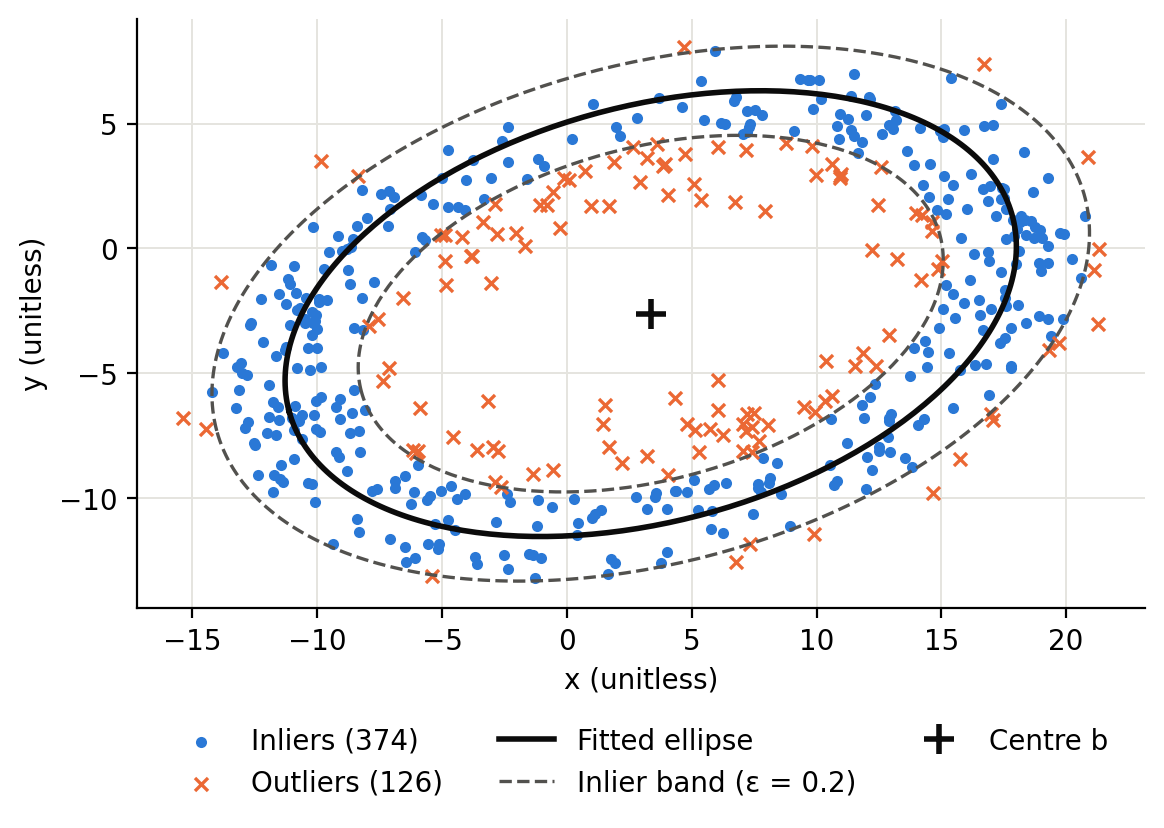
\includegraphics[width=0.8\linewidth]{q2_ransac_ellipse.png}
    \caption{RANSAC result for $N = 500$ points, 1000 iterations and $\varepsilon = 0.2$ (seed 0), showing the inliers, outliers, fitted ellipse, inlier band and centre $\vect{b}$. Axes are unitless. The ellipse is drawn directly from the fitted $\mat{Q}$ and $\vect{b}$ by a separate helper script.}
    \label{fig:q2b}
\end{figure}

\subsection*{2(c) Effect of dataset size, iterations and threshold [10 pts] \quad (max 100 words)}

\begin{table}[h!]
    \centering
    \footnotesize
    \begin{tabular}{llccccccc}
\toprule
Varied & Value & Runs & Inliers (\%) & $b_x$ & $b_y$ & Major & Minor & Time (s) \\
\midrule
$N$ & 50 & 10/10 & 78.2 $\pm$ 3.8 & 2.87 $\pm$ 0.79 & -2.70 $\pm$ 0.83 & 15.65 $\pm$ 0.98 & 7.70 $\pm$ 0.62 & 0.066 \\
 & 100 & 10/10 & 77.2 $\pm$ 3.6 & 2.93 $\pm$ 0.65 & -2.52 $\pm$ 0.66 & 15.22 $\pm$ 0.60 & 7.77 $\pm$ 0.45 & 0.071 \\
 & 500 & 10/10 & 73.5 $\pm$ 1.9 & 3.52 $\pm$ 0.36 & -2.48 $\pm$ 0.39 & 15.54 $\pm$ 0.52 & 7.55 $\pm$ 0.42 & 0.085 \\
 & 2000 & 10/10 & 72.6 $\pm$ 0.5 & 3.41 $\pm$ 0.44 & -2.69 $\pm$ 0.32 & 15.59 $\pm$ 0.50 & 7.64 $\pm$ 0.38 & 0.198 \\
 & 4999 & 10/10 & 72.2 $\pm$ 1.1 & 3.48 $\pm$ 0.56 & -2.56 $\pm$ 0.30 & 15.77 $\pm$ 0.48 & 7.57 $\pm$ 0.23 & 0.288 \\
\midrule
Iterations & 10 & 10/10 & 61.0 $\pm$ 8.8 & 3.10 $\pm$ 1.93 & -2.76 $\pm$ 1.13 & 16.46 $\pm$ 1.44 & 7.71 $\pm$ 0.78 & 0.001 \\
 & 50 & 10/10 & 67.1 $\pm$ 5.1 & 3.94 $\pm$ 1.10 & -2.26 $\pm$ 0.78 & 15.84 $\pm$ 1.07 & 7.64 $\pm$ 0.58 & 0.005 \\
 & 200 & 10/10 & 70.9 $\pm$ 2.1 & 3.79 $\pm$ 0.69 & -2.55 $\pm$ 0.48 & 15.52 $\pm$ 0.83 & 7.49 $\pm$ 0.70 & 0.019 \\
 & 1000 & 10/10 & 73.5 $\pm$ 1.9 & 3.52 $\pm$ 0.36 & -2.48 $\pm$ 0.39 & 15.54 $\pm$ 0.52 & 7.55 $\pm$ 0.42 & 0.082 \\
 & 5000 & 10/10 & 74.9 $\pm$ 1.7 & 3.24 $\pm$ 0.40 & -2.80 $\pm$ 0.24 & 15.30 $\pm$ 0.36 & 7.72 $\pm$ 0.36 & 0.419 \\
\midrule
$\varepsilon$ & 0.02 & 10/10 & 12.0 $\pm$ 1.3 & 3.78 $\pm$ 6.88 & -3.26 $\pm$ 5.28 & 19.11 $\pm$ 5.77 & 9.95 $\pm$ 3.79 & 0.088 \\
 & 0.05 & 10/10 & 25.8 $\pm$ 2.3 & 4.50 $\pm$ 7.80 & -3.20 $\pm$ 5.21 & 19.93 $\pm$ 6.52 & 9.94 $\pm$ 3.42 & 0.082 \\
 & 0.1 & 10/10 & 45.1 $\pm$ 2.7 & 4.45 $\pm$ 7.81 & -3.14 $\pm$ 5.21 & 19.81 $\pm$ 6.62 & 9.83 $\pm$ 3.48 & 0.080 \\
 & 0.2 & 10/10 & 73.5 $\pm$ 1.9 & 3.52 $\pm$ 0.36 & -2.48 $\pm$ 0.39 & 15.54 $\pm$ 0.52 & 7.55 $\pm$ 0.42 & 0.082 \\
 & 0.5 & 10/10 & 99.2 $\pm$ 0.4 & 3.34 $\pm$ 0.69 & -2.58 $\pm$ 0.39 & 15.02 $\pm$ 1.29 & 7.88 $\pm$ 0.38 & 0.080 \\
 & 1.0 & 10/10 & 100.0 $\pm$ 0.0 & 1.82 $\pm$ 2.50 & -3.26 $\pm$ 2.07 & 17.64 $\pm$ 3.07 & 7.55 $\pm$ 0.66 & 0.079 \\
\bottomrule
\end{tabular}

    \caption{Results for each setting over 10 seeds, as mean $\pm$ standard deviation across the runs that returned a model. ``Runs'' is the number of seeds that returned a model. $b_x$ and $b_y$ are the components of the centre, ``Major'' and ``Minor'' are the semi-axes, and all are unitless.}
    \label{tab:q2c}
\end{table}

\begin{figure}[h!]
    \centering
    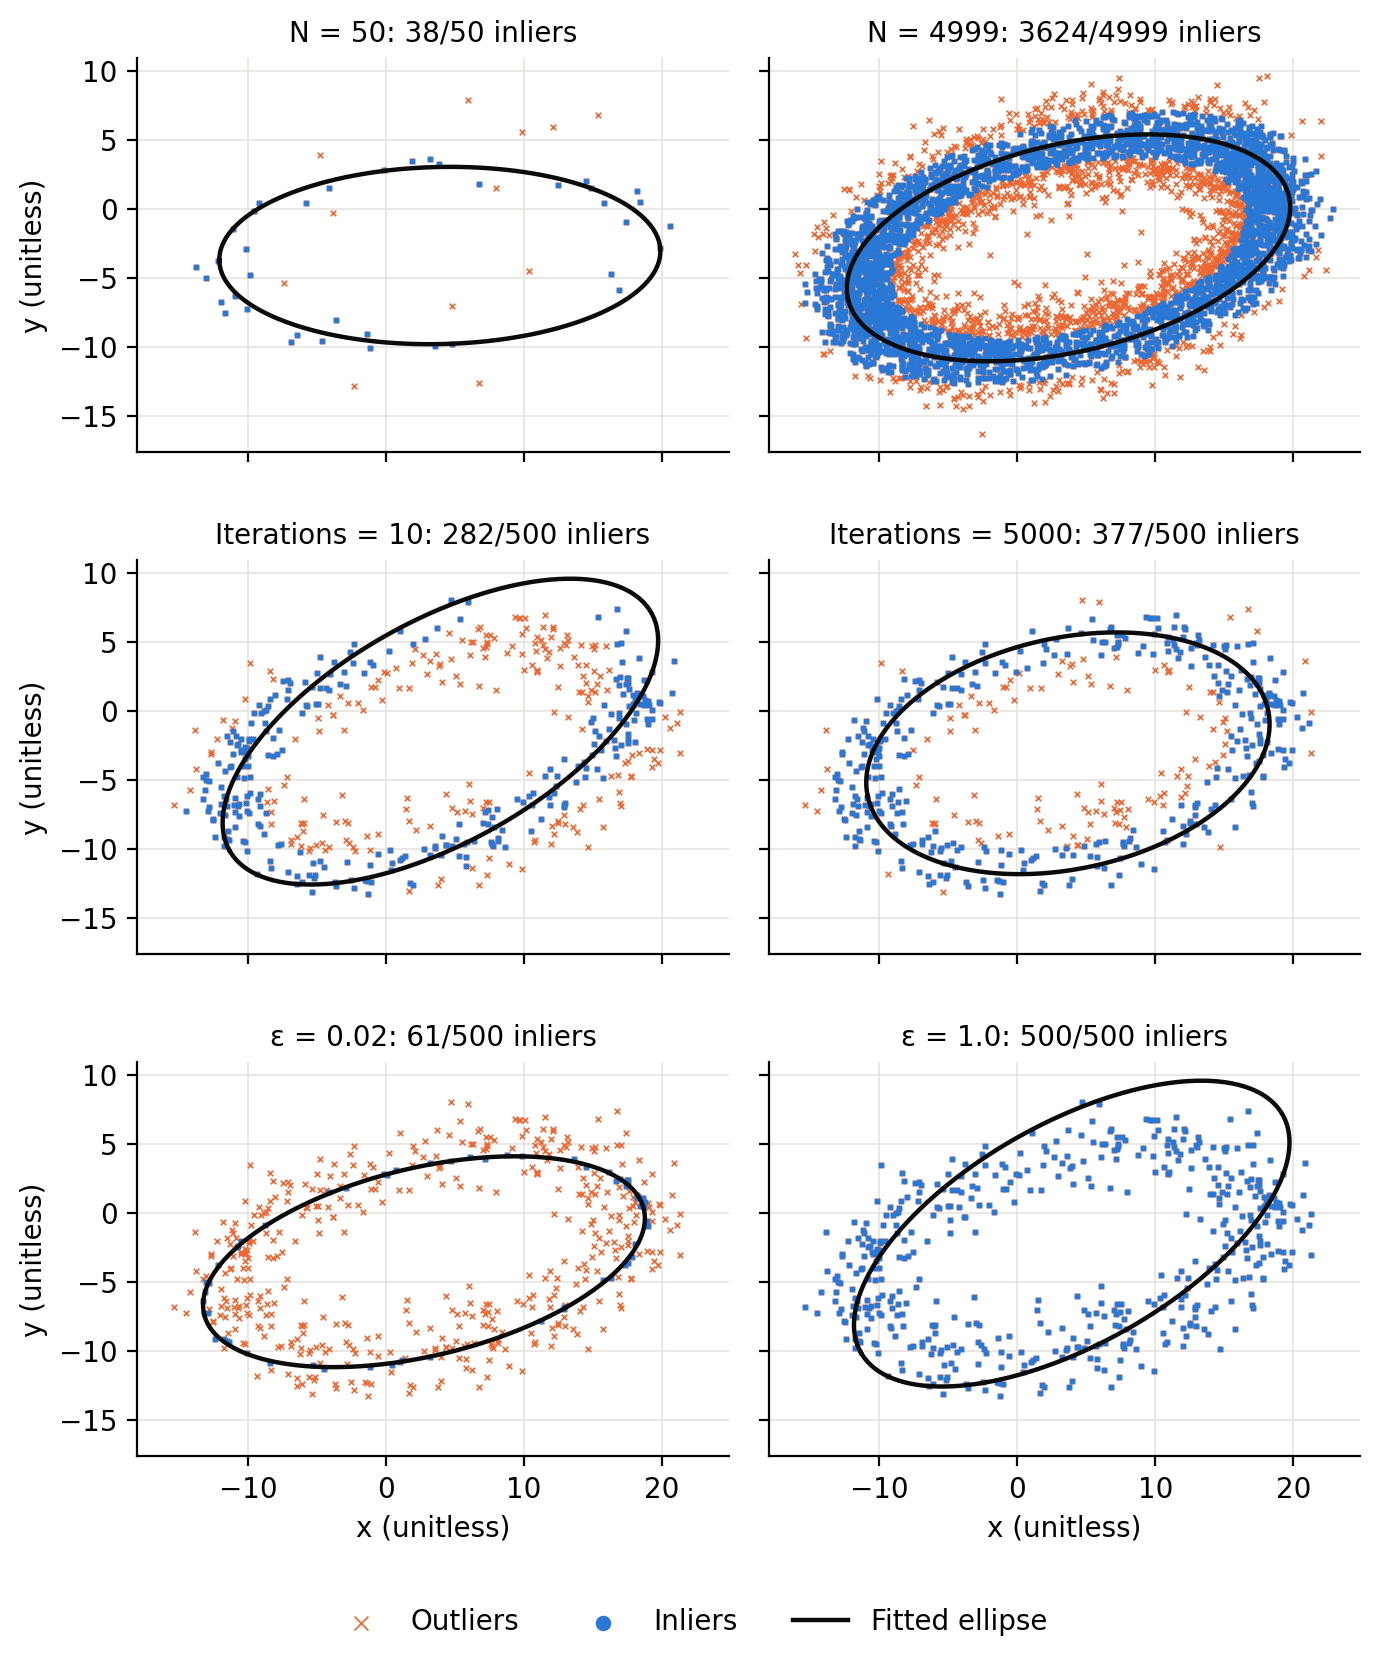
\includegraphics[width=0.85\linewidth]{q2c_extremes.png}
    \caption{Fitted ellipse at the smallest and largest value of each setting (seed 0), with the other two settings at their baseline values. Axes are unitless.}
    \label{fig:q2c}
\end{figure}

Table~\ref{tab:q2c} summarises ten seeds per setting, and Figure~\ref{fig:q2c} shows each setting's extremes, with the others at baseline.

\textbf{Points ($N$):} the inlier percentage stays roughly steady, and the centre stabilises up to $N = 500$; beyond that, gains are small while runtime grows.

\textbf{Iterations:} too few often miss an all-inlier sample, so fits vary between seeds. Beyond about 1000, results stop improving and only runtime grows.

\textbf{Threshold $\varepsilon$:} small $\varepsilon$ rejects noisy true points, giving few inliers and an unstable fit. Large $\varepsilon$ accepts outliers, inflating the inlier count and biasing the ellipse. $\varepsilon \approx 0.2$ balanced both.

% \begin{figure}[h]
%   \centering
%   \includegraphics[width=0.7\linewidth]{q2c_example.png}
%   \caption{...}
%   \label{fig:q2c}
% \end{figure}

% =====================================================================
\clearpage
\section{Bayesian Filter for Tracking Moo-Deng's Behavior I (32 pts)}

\subsection*{3(a) Probability of sequence (2,3,3,1) [4 pts] \quad (max 50 words)}

\begin{equation*}
    P = p(2|1) \cdot p(3|2) \cdot p(3|3) \cdot p(1|3) = 0.4 \times 0.4 \times 0.7 \times 0.2 = 0.0224 \ (2.24\%)
\end{equation*}
By the Markov property, each move depends only on the current zone, so the probability of the whole path is the product of the one-step transition probabilities: Feeding$\to$Resting (0.4), Resting$\to$Playground (0.4), Playground$\to$Playground (0.7), Playground$\to$Feeding (0.2).

\subsection*{3(b) Transition matrix $\mat{A}$ [5 pts] \quad (max 50 words)}

\begin{equation*}
    \mat{A} = \begin{bmatrix} 0.6 & 0.2 & 0.2 \\ 0.4 & 0.4 & 0.1 \\ 0.0 & 0.4 & 0.7 \end{bmatrix}
    \qquad \text{(columns: from F, R, P; rows: to F, R, P)}
\end{equation*}
Since $\vect{x}_{k+1} = \mat{A}\vect{x}_k$, entry $\mat{A}_{ij} = p(A_{k+1} = i \mid A_k = j)$, so column $j$ lists where Moo-Deng goes from zone $j$. Each column comes from one behaviour bullet and sums to 1. $\mat{A}_{31} = 0$ because she never moves from Feeding directly to Playground.

\subsection*{3(c) Stationary probabilities [8 pts]}

A stationary distribution does not change under a transition, so $\vect{x}^* = \mat{A}\vect{x}^*$, which is equivalent to $(\mat{A} - \mat{I})\vect{x}^* = \vect{0}$, together with $x_1 + x_2 + x_3 = 1$.
\begin{equation*}
    \mat{A} - \mat{I} = \begin{bmatrix} -0.4 & 0.2 & 0.2 \\ 0.4 & -0.6 & 0.1 \\ 0.0 & 0.4 & -0.3 \end{bmatrix}
\end{equation*}
The three rows of $(\mat{A} - \mat{I})$ sum to zero, so only two of the equations are independent. The normalisation $x_1 + x_2 + x_3 = 1$ supplies the third.

\begin{itemize}
    \item Row 1: $-0.4x_1 + 0.2x_2 + 0.2x_3 = 0$, which gives $2x_1 = x_2 + x_3$.
    \item Substitute $x_2 + x_3 = 1 - x_1$: $2x_1 = 1 - x_1$, so $x_1 = 1/3$.
    \item Row 2: $0.4x_1 - 0.6x_2 + 0.1x_3 = 0$. With $x_1 = 1/3$: $4/3 - 6x_2 + x_3 = 0$, so $x_3 = 6x_2 - 4/3$.
    \item Substitute into $x_2 + x_3 = 2/3$: $7x_2 - 4/3 = 2/3$, so $x_2 = 2/7$.
    \item $x_3 = 6(2/7) - 4/3 = 8/21$.
\end{itemize}
\begin{equation*}
    \vect{x}^* = \begin{bmatrix} 1/3 \\ 2/7 \\ 8/21 \end{bmatrix} = \begin{bmatrix} 7/21 \\ 6/21 \\ 8/21 \end{bmatrix} \approx \begin{bmatrix} 0.333 \\ 0.286 \\ 0.381 \end{bmatrix}
\end{equation*}

Check with row 3: $0.4(2/7) - 0.3(8/21) = 8/70 - 8/70 = 0$ $\checkmark$. Equivalently, $\vect{x}^*$ is the eigenvector of $\mat{A}$ for eigenvalue 1, normalised to sum to 1. $\mat{A}^{100}[1, 0, 0]^\top$ gives the same values, so the long-run result does not depend on the starting zone.

Over the long run, Moo-Deng spends about 33\% of her time feeding, 29\% resting and 38\% in the playground.

\subsection*{3(d) Measurement matrix $\mat{C}$ [5 pts] \quad (max 50 words)}

\begin{equation*}
    \mat{C} = \begin{bmatrix} 0.80 & 0.20 & 0.05 \\ 0.10 & 0.70 & 0.10 \\ 0.10 & 0.10 & 0.85 \end{bmatrix}
    \qquad \text{(columns: true zone F, R, P; rows: displays F, R, P)}
\end{equation*}
Since $[p(\vect{y} = \vect{e}_1),\ p(\vect{y} = \vect{e}_2),\ p(\vect{y} = \vect{e}_3)]^\top = \mat{C}\vect{x}_k$, entry $\mat{C}_{ij} = p(\text{display } i \mid \text{true zone } j)$. Column $j$ is the sensor bullet for zone $j$, and each column sums to 1. The diagonal holds the accuracies; the off-diagonal entries are the misreadings.

\subsection*{3(e) Bayesian filter state estimator [10 pts]}

This applies the general Bayes filter (Localization III, slide 59) to 3 discrete states with no control input.

\textbf{Prediction step.} By total probability and the Markov property:
\begin{equation*}
    \bar{x}_k(i) = \sum_j p(A_k = i \mid A_{k-1} = j)\, x_{k-1}(j) \quad\Longrightarrow\quad \bar{\vect{x}}_k = \mat{A}\vect{x}_{k-1}
\end{equation*}

\textbf{Correction step.} By Bayes' rule, with the measurement depending only on the current state:
\begin{equation*}
    x_k(i) = \eta \cdot p(\vect{y}_k \mid A_k = i) \cdot \bar{x}_k(i)
\end{equation*}
For the reading $\vect{y}_k$ actually received, $p(\vect{y}_k \mid A_k = i)$ for $i = 1, 2, 3$ is the row of $\mat{C}$ picked out by $\vect{y}_k$, which is the vector $\mat{C}^\top\vect{y}_k$. In matrix form:
\begin{equation*}
    \vect{x}_k = \eta \cdot \operatorname{diag}(\mat{C}^\top\vect{y}_k)\, \mat{A}\vect{x}_{k-1}, \qquad \eta = \frac{1}{\vect{y}_k^\top\mat{C}\mat{A}\vect{x}_{k-1}} = \frac{1}{\sum_i [\operatorname{diag}(\mat{C}^\top\vect{y}_k)\,\mat{A}\vect{x}_{k-1}]_i}
\end{equation*}
$\eta$ normalises $\vect{x}_k$ so that it sums to 1. Its denominator is $p(\vect{y}_k \mid \vect{y}_{1:k-1})$, the predicted probability of the reading.

\textbf{State estimate.} Take the most likely zone: $\hat{A}_k = \arg\max_i x_k(i)$.

\textbf{With numbers.} The likelihood vector $\mat{C}^\top\vect{y}_k$ for each possible reading is:
\begin{center}
\begin{tabular}{ll}
    \toprule
    Reading $\vect{y}_k$ & $\mat{C}^\top\vect{y}_k$ \\
    \midrule
    Feeding $[1, 0, 0]^\top$ & $[0.80, 0.20, 0.05]^\top$ \\
    Resting $[0, 1, 0]^\top$ & $[0.10, 0.70, 0.10]^\top$ \\
    Playground $[0, 0, 1]^\top$ & $[0.10, 0.10, 0.85]^\top$ \\
    \bottomrule
\end{tabular}
\end{center}

\textbf{Example.} Take $\vect{x}_{k-1} = [1, 0, 0]^\top$ (known to be Feeding) and a Feeding reading.
\begin{itemize}
    \item Prediction: $\bar{\vect{x}}_k = \mat{A}\vect{x}_{k-1} = [0.6, 0.4, 0]^\top$.
    \item Multiply by the likelihood $[0.80, 0.20, 0.05]^\top$ element-wise: $[0.48, 0.08, 0]^\top$. The sum is 0.56, so $\eta = 1/0.56$.
    \item Normalise: $\vect{x}_k = [0.857, 0.143, 0]^\top$, so $\hat{A}_k = 1$ (Feeding).
\end{itemize}

\textbf{Algorithm} (one step per observation):
\begin{enumerate}
    \item Predict: $\bar{\vect{x}}_k = \mat{A}\vect{x}_{k-1}$
    \item Update: $\tilde{\vect{x}}_k = (\mat{C}^\top\vect{y}_k) \odot \bar{\vect{x}}_k$ ($\odot$ = element-wise product)
    \item Normalise: $\vect{x}_k = \tilde{\vect{x}}_k / (\vect{1}^\top\tilde{\vect{x}}_k)$
    \item Estimate: $\hat{A}_k = \arg\max \vect{x}_k$
\end{enumerate}

% =====================================================================
\clearpage
\section{Bayesian Filter for Tracking Moo-Deng's Behavior II (20 pts)}

\subsection*{4(a) \texttt{moodeng\_behavior\_update} [6 pts] \quad (max 50 words)}
% TODO

\subsection*{4(b) \texttt{sensor\_measurement} [6 pts]}
% TODO

\subsection*{4(c) \texttt{sim\_moodeng} state estimator [8 pts]}
% TODO -- include plots (axes labelled with units, captions)

\end{document}
